\documentclass[a4paper]{article}
\usepackage[warn]{mathtext}
\usepackage[utf8]{inputenc}
\usepackage[T2A]{fontenc}
\usepackage[english,russian]{babel}
\usepackage{indentfirst}
\usepackage{misccorr}
\usepackage{subcaption}
\captionsetup{compatibility=false}
\usepackage{geometry}
\geometry{verbose,a4paper,tmargin=2cm,bmargin=2cm,lmargin=1.5cm,rmargin=1.5cm}
\usepackage{graphicx}
\usepackage{wrapfig}
\usepackage{amsmath}
\usepackage{fancyhdr}
\usepackage{floatflt}
\usepackage{float}
\usepackage{amssymb}
\usepackage{color}
\usepackage{lscape}
\usepackage{hvfloat}
\usepackage{amsfonts}
\usepackage{euscript}
\usepackage{newunicodechar}
\usepackage{booktabs}

\begin{document}
\newcommand{\apple}{\char"F8FF}



\begin{titlepage}
    \vspace*{4cm}
	\centering
    {\scshape\LARGE Московский физико-технический институт\par}
	\vspace{1cm}
	{\scshape\Large Лабораторная работа по общей физике № 10.1\par}
	\vspace{1cm}
    {\huge\bfseries  Электронный парамагнитный резонанс \par}
	\vspace{2cm}
	\vfill
\begin{flushright}
	{\large Выполнила студентка Б01-907}\par
	\vspace{0.3cm}
	{\LARGE Юлия Прохорова}
\end{flushright}
	
	\vfill
Долгопрудный, 2021
% Bottom of the page
\end{titlepage}

\pagestyle{fancy} 
\fancyhead[L]{№ 10.1}
\fancyhead[R]{Юля Прохорова, Б01-907}
\fancyhead[C]{}
\fancyfoot[C]{ \noindent\rule{\textwidth}{0.4pt} \thepage }

\tableofcontents

\newpage


\section{Цель работы}

Исследуется электронный парамагнитный резонанс в молекуле ДФПГ, определяется $g-$фактор электрона, измеряется ширина линии ЭПР.
\section{Оборудование}
Блок питания, вольтметр, трансформатор ЛАТР, милливольтметр, осциллограф, генератор МГц диапазона.

\section{Теория}

Энергетический уровень электрона в присутствии магнитного поля $B$ расщепляется на два подуровня, расстояние между которыми равно 
\begin{equation}
    \varDelta E = E_2 - E_1 = 2\mu B \label{eq1}
\end{equation}

Здесь $\mu$ - абсолютная величинапроекции магнитного момента на направение поля.
Между уровнями возможны переходы - в случае, если внешнее электромагнитное поле имеет нужную частоту и направление.\\

Резонансное значение частоты:
\begin{equation}
    \hbar \omega_0 = \varDelta E = 2\mu B \label{eq2}
\end{equation}

возбуждение электронных резонансных переходов электромагнитным полем, имеющим частоту \ref{eq2}, называется электронно парамагнитного резонанса (ЭПР).
ЭПР возникает из-за переворота спина электронов под действием под действием высокочастотного электромагнитного поля.  Сигнал электронного парамагнитного резонанса наблюдается лишь на неспаренных электронных образцах.

В свободных атомах электрические поля, действующие на атомные электроны, - центральные, и момент количества движения электрона $J$ сохранятеся. Здесь орбитальное квантовое число $L$ является квантовым, сохраняется и оказывается практически точным $J$. \\

Рассмотрим структурную формулу ЭПР свободного радикала ДФПГ (дифенилприкрилгидразил):

\begin{wrapfigure}[17]{l}{145pt}
    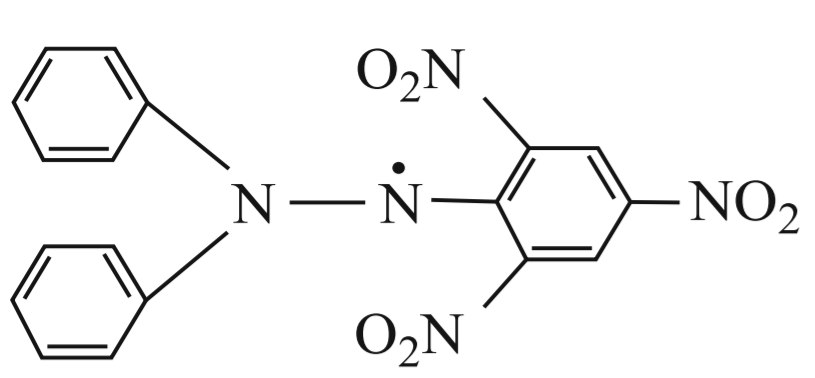
\includegraphics[scale = 0.2]{pic1.png}
    \caption{Структурная формула молекулы ДФПГ}
    \label{pic1}
\end{wrapfigure}

Неспаренные электроны радикалов приводят к их повышенной химическойактивности. \\
В отсутствие высокочастотного поля заселенность уровней определяется температурой и описывается формулой Больцмана:

\begin{equation}
    \frac{N_в}{N_н} = exp(-\frac{\varDelta E}{k_БTT}) \label{eq3}
\end{equation}

В присутствии поля - соотношение \ref{eq3} нарушается. Восстановление теплового равновесия осуществляется благодаря передаче энергии возбуждения другим степеям свободы тела (благодаря спин-спиновому и спин-решеточному взаимодействиям). \\
Оба типа взаимодействия способствуют релаксации - переходу из возбужденного состояния в основное. Ширина уровня связана со временем релаксации соотношением неопределенностей:

\begin{equation}
    \varDelta E \approxeq \frac{\hbar}{\tau}, \; \varDelta \omega \approxeq \frac{1}{\tau} \label{eq4}
\end{equation}

В работе требуется получить сигнл ЭПР на кристалах ДФПГ и определить значение $g-$фактора для электрона. 

Связь магнитного $\mu$ и механического $M$ моментов:

\begin{equation}
    \mu = \gamma M \label{eq5}
\end{equation}

\begin{equation}
    \frac{\mu}{\mu_Б} = \frac{gM}{\hbar} \label{eq6} 
\end{equation}

Запишем \ref{eq6} в проекциях на любое направление:

\begin{equation}
    \frac{\mu}{\mu_Б} = \frac{gs\hbar}{\hbar}, \label{eq7} 
\end{equation}
 где $s=1/2$ - спин электрона. Используя соотношение \ref{eq2} выразим $g-$фактор:

\begin{equation}
    g = \frac{\hbar \omega_0}{\mu_Б B} \label{eq8}
\end{equation}

Тк у ДФПГ практически отсутствует орбитальный магнетизм - ЭПР на неспаренных электронах происходит почти как на свобоных частицах.

\section{Экспериментальная установка}

Для наблюдения ЭПР необходимы чувствительные радиоспектр. Охлаждая ДФПГ, можно исследовать зависимость шириы линии поглощения от температуры и установить характер уширения: спин-спиновыйили спин-решеточный. Для наблюдения ЭПР нужно поместить исследуемое вещество в магнитное поле и измерить поглощение электромагнитного излучения. Заметный эффект получается получить, применяя устройства, сосредотачивающие энергию электромагнитного поля в объеме образца, например, колебательный контур, в катушку которог помещено исследуемое вещество. Наблюдение ЭПР состоит в савнении добротности катушки в условиях резонанса и при расстройке, когда условие резонанса не выполняется. Удобнее менять магнитное поле, так как при этом в измерительной цепи не происходит никаких изменений и меняются только потери, связанные с ЭПР. 


\begin{figure}[H]
    \center{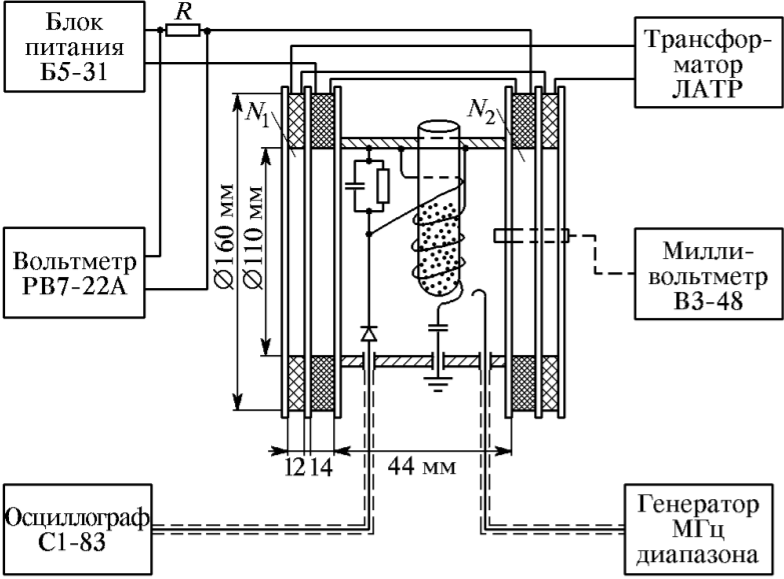
\includegraphics[scale=0.4]{pic2.png}}
    \caption{Блок-схема установки для наблюдения ЭПР. Измерение постоянного и переменного токов через катушки $N_2$ производится с помощью вольтметра $PB7-22A$ и сопротивления $R = 10 Ом$, включенного в цепь катушек.}
    \label{pic2}
    \end{figure}

% \begin{wrapfigure}[23]{l}{300pt}
%     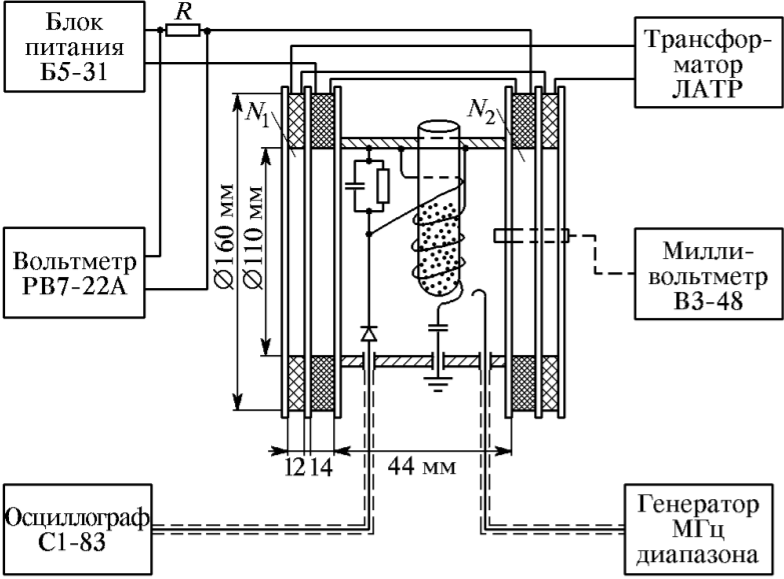
\includegraphics[scale = 0.4]{pic2.png}
%     \caption{Блок-схема установки для наблюдения ЭПР. Измерение постоянного и переменного токов через катушки $N_2$ производится с помощью вольтметра $PB7-22A$ и сопротивления $R = 10 Ом$, включенного в цепь катушек.}
%     \label{pic2}
% \end{wrapfigure}

\begin{figure}[H]
    \begin{center}
    \begin{minipage}[h]{0.45\linewidth}
        \begin{center}
            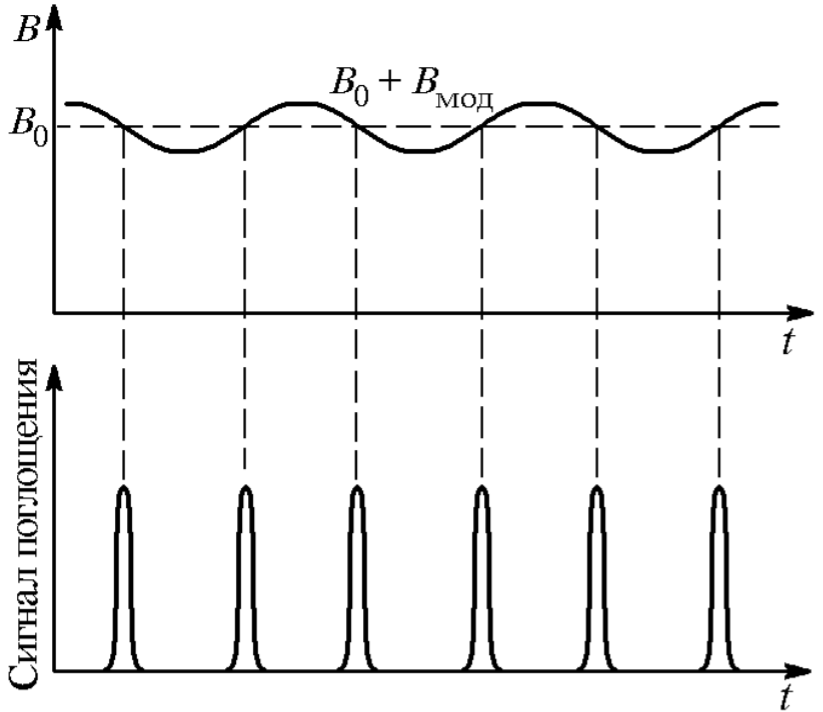
\includegraphics[scale = 0.2]{pic3.png}
            \caption{Сигналы полголощения электронного парамагнитного резонанса при переменной развертке луча осциллографа, когда основное магнитное поле точно подобрано.}
            \label{p2}  
        \end{center}
    \end{minipage}
    \hfill
    \begin{minipage}[h]{0.45\linewidth}
        \begin{center}
            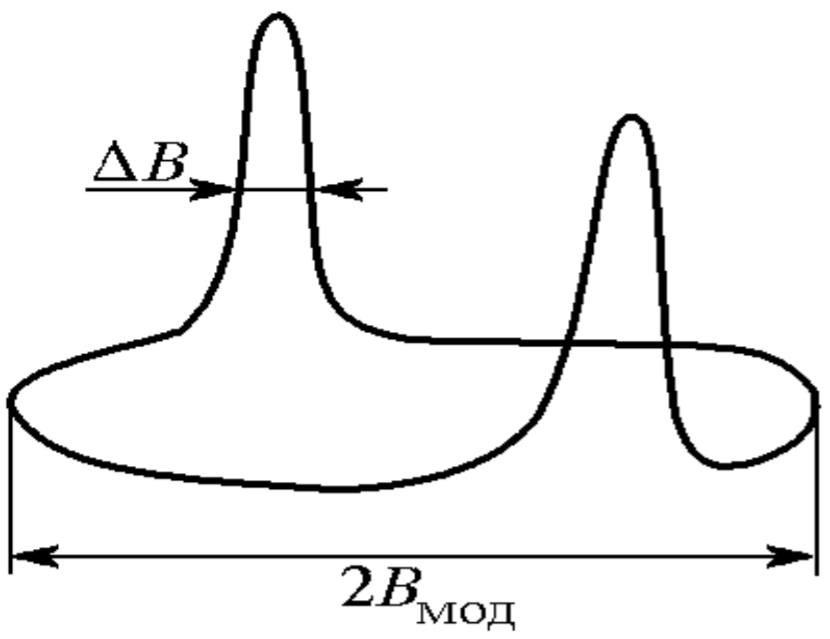
\includegraphics[scale = 0.2]{pic4.png}
            \caption{Сигналы поглощения ЭПР при развертке луча осциллографа напряжением модулирующих катушек.}
            \label{p3}
        \end{center}
    \end{minipage}
    \end{center}
    \end{figure}

% \begin{wrapfigure}[15]{l}{145pt}
%     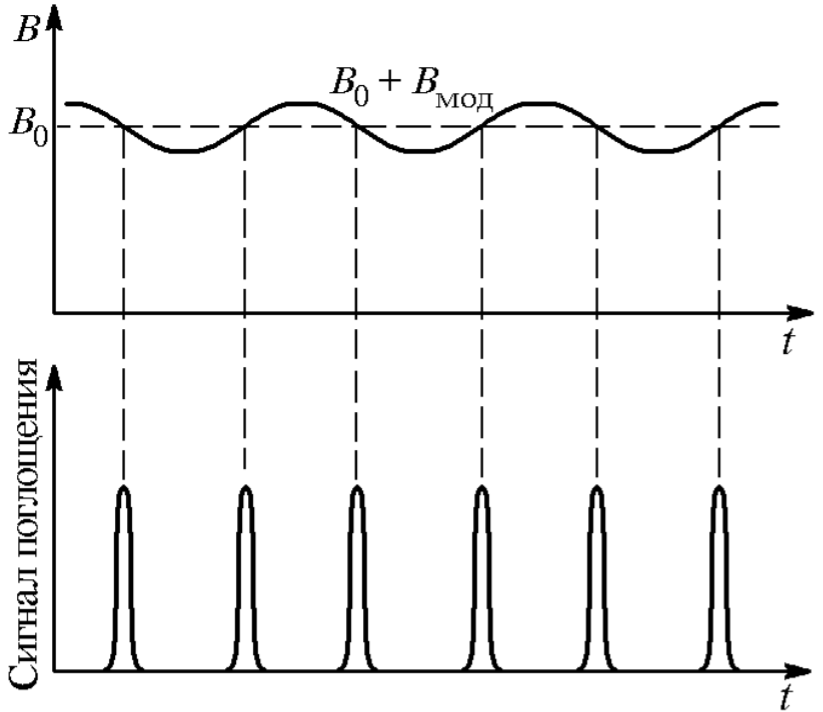
\includegraphics[scale = 0.2]{pic3.png}
%     \caption{Сигналы полголощения электронного парамагнитного резонанса при переменной развертке луча осциллографа, когда основное магнитное поле точно подобрано.}
%     \label{pic3}
% \end{wrapfigure}

Контур заключен в латунный посеребренный изнутри контейнер. Ампула с исследуемым образцом вставляется в катушку индуктивности контура. Основное магнитное поле в образце создается с помощью двух соосно расположенных катушек, питаемых от источника постоянного тока. Небольшое модулированное поле создается при помощи дополнительных катушек. 
При наступлении ЭПР поглощение энергии  в образце увеличивается, добротность колебательного контура падает, и амплитуда колебаний в контуре уменьшается. 

% \begin{wrapfigure}[13]{r}{145pt}
%     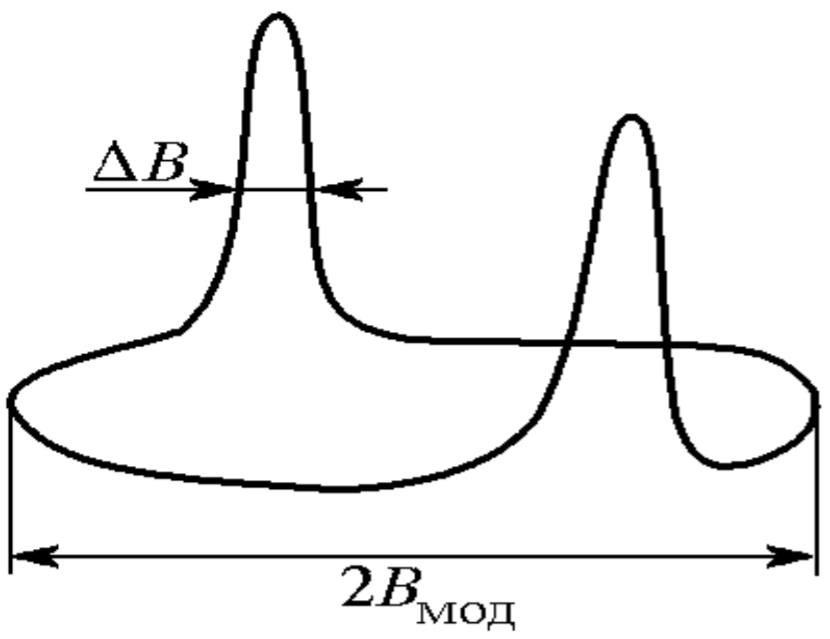
\includegraphics[scale = 0.2]{pic4.png}
%     \caption{Сигналы поглощения ЭПР при развертке луча осциллографа напряжением модулирующих катушек.}
%     \label{pic2}
% \end{wrapfigure}

Если основное поле $B$ подобрано точно, то на экране осциллографа с временной разверткой сигналы электронного парамагнитного резонанса распологаются через равные промежутки.\\
Удобно наблюдать сигнал электронного парамагнитного резонанса, подавая горизонтальную развертку усилителя сигнал с модулирующих катушек.Наличие двух сигналов объясняется сдвигом фаз между напряжением и током модулирующик катушек.


\section{Ход работы}

\subsection{Получение сигнала ЭПР на свободном радикале ДФПГ и измерение $g-$фактора электрона.}

\begin{enumerate}
    \item Настроим генератор на резонансную частоту контура $\nu_{рез} = (128,5 \pm 0,4)$МГц. При точной настройке генератора на частоту контура амплитуда колебаний на экране осциллографа - наибольшая. 
    \item Включим питание основных катушек от источника постоянного тока и питание модулирующих катушек. Установим а модулирующей катушке напряжение около $50В$.
    \item Включим временную развертку осциллографа.
    \item Плавно меняя реостатом величину тока, проходящего через основные катушки, найдём сигнал ЭПР.Отрегулировали величину тока так, чтобырасстояние между пиками резонанса на экране осциллографа было одинаковым.
    
    \begin{table}[H]
        \begin{center}
            \begin{tabular}{|c|c|}
                \hline
                $V_R$, мВ & $V_{пр}$, мВ \\  \hline
                24,65    & 4,56 $\pm$ 0,15\\ \hline
                30,85    & 5,63 $\pm$ 0,16\\ \hline
                37,18    & 6,78 $\pm$ 0,19\\ \hline
                43,35    & 7,84 $\pm$ 0,21\\ \hline
                49,61    & 9,01 $\pm$ 0,27\\ \hline
                55,50    & 10,07 $\pm$ 0,25\\ \hline
                61,60    & 11,20 $\pm$ 0,28\\ \hline
                68,10    & 12,21 $\pm$ 0,28\\ \hline
                74,28    & 13,48 $\pm$ 0,31 \\ \hline
                \end{tabular}
                \caption{$V_{пр}(V_R)$}
        \end{center}
    \end{table}
   
    \begin{figure}[H]
    \center{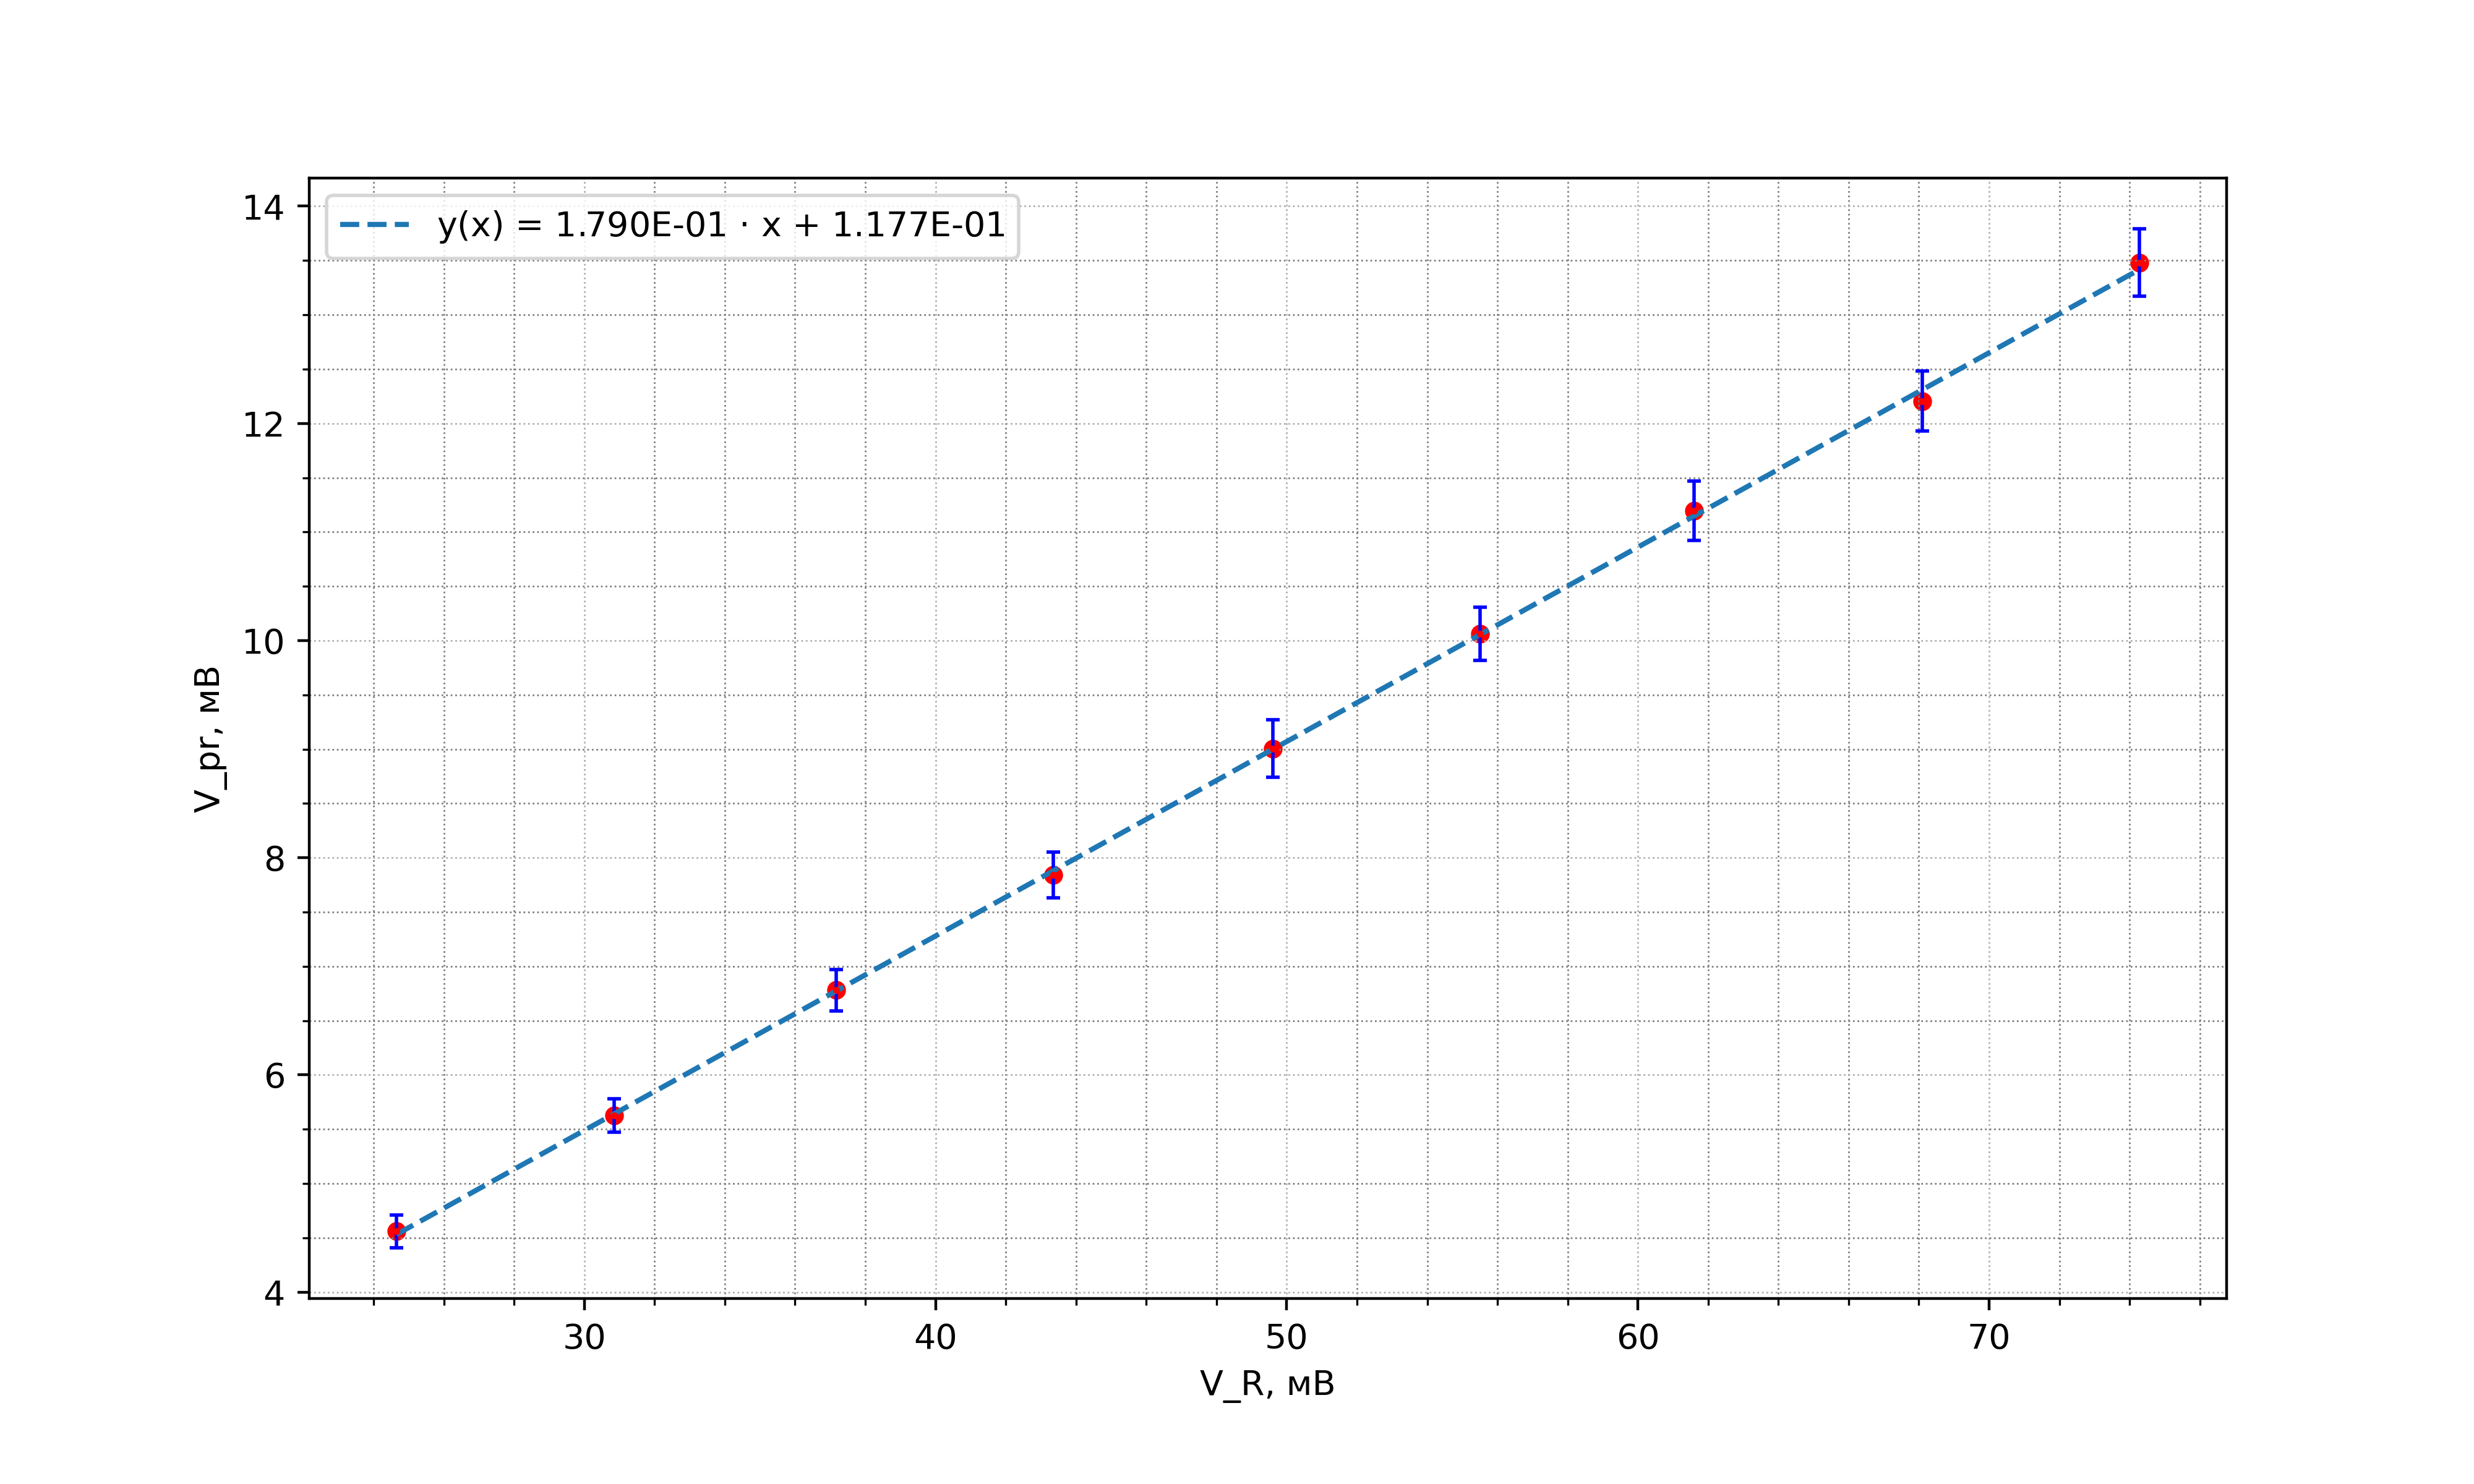
\includegraphics[scale=0.5]{V.png}}
    \caption{Колибровка }
    \label{V}
    \end{figure}

    \item Из графика получаем $V_{pr} = (11,1 \pm 0,1)$мВ
    
    \item Посчитаем индукцию основного магнитного поля :
    
    \begin{equation}
        B_0 = \frac{V_{пр}}{N_{пр}S_{пр}\omega_0} \label{eq9},
    \end{equation}    
    где $N_{пр} = 46$, $S_{пр} = \pi d^2$, $d = 14,6 \pm 0,1$ мм.
    \begin{equation}
        B_0 = (4,5 \pm  0.1)мТл \label{eq10}, 
    \end{equation} 
    где 
    \begin{equation}
        \sigma_{B_0} = \sqrt{(\frac{\partial B_0}{\partial V_{pr}})^2\sigma_{V_{pr}}^2+(\frac{\partial B_0}{\partial d})^2\sigma^2_{d}}  \label{eq11}
    \end{equation}

    \item Для измерения $g-$фактора электрона, нашли резонансные значения частоты $\omega_0$ и индукции $B_0$.  Определим $g$ по формуле:
    
    \begin{equation}
        g = \frac{h \nu_0}{\mu_B B_0} = 2.00 \pm 0.09 \label{eq12}, 
    \end{equation}
    где 
    \begin{equation}
        \sigma_{g} = \sqrt{(\frac{\partial g}{\partial \nu_0})^2\sigma_{\nu_0}^2+(\frac{\partial g}{\partial B_0})^2\sigma^2_{B_0}}  \label{eq13}
    \end{equation}
    \item Полученный значение $g-фактора$ электрона отлично сходится с теоретическим в пределах погрешности - $g = 2.004$.
\end{enumerate}

\subsection{Определение ширины линии ЭПР}
\begin{enumerate} 
    \item Переключим осциллограф на развертку от модуляционных катушек. Длина развертки соответствует удвоенной амплитуде модулирующего поля $2L = (7,5 \pm 0,25) дел$.
    \item На полувысоте $\varDelta L = (1,5 \pm 0,3) дел$. Значение $V_{pr} = (1,13 \pm 0,02)$мВ.
    \item Рассчитаем $B_{мод}$ по формуле:
    \begin{equation}
        B_{мод} = \frac{\sqrt{2}V_{pr}}{SN\omega_0} = (0,165 \pm 0.004 )мТл\label{eq14}, 
    \end{equation}
    где 
    \begin{equation}
        \sigma_{B_{мод}} = \sqrt{(\frac{\partial B_{мод}}{\partial V_{pr}})^2\sigma_{V_{pr}}^2+(\frac{\partial B_{мод}}{\partial d})^2\sigma_{d}^2}  \label{eq13}
    \end{equation}
    \item Полуширину на полувысоте линии резонансного поглощения рассчитаем по формуле:
        \begin{equation}
           \varDelta B = \frac{2 B_{мод}\varDelta L}{L} = (0.066 \pm 0.013) мТл 
        \end{equation}
        где 
        \begin{equation}
            \sigma_{ \varDelta B} = \sqrt{(\frac{\partial \varDelta B}{\partial \varDelta L})^2\sigma_{\varDelta L}^2+(\frac{\partial \varDelta B}{\partial L})^2\sigma_{L}^2+(\frac{\partial \varDelta B}{\partial B_{мод}})^2\sigma^2_{B_{мод}}}  \label{eq13}
        \end{equation}
\end{enumerate}

\section{Вывод}
 В ходе работы исследовали ЭПР в молекуле ДФПГ, определили $g-$фактор этектрона $g = 2.00 \pm 0.09$ и измерили ширину линии ЭПР $\varDelta B = 0.165 \pm 0.004$ мТл.

\section{Литература}
Игошин Ф.Ф., Самарский Ю.А., Ципенюк Ю.М.  - Лабораторный практикум по общей физике: Учеб. пособие для вузов. Т. 3 Квантовая физика. 

\end{document}